% Maritime Radar Tracking Paper - AIAA Format with TikZ Figures
\documentclass[conf]{new-aiaa}
%\usepackage[margin=1in]{geometry} % Handled by class
\usepackage{graphicx}
\let\Bbbk\relax
\usepackage{amsmath,amssymb}
\usepackage{booktabs}
\usepackage{hyperref}
\usepackage{tikz}
\usetikzlibrary{positioning,shapes,arrows.meta,patterns,calc,decorations.pathreplacing}
\usepackage{authblk}
\usepackage{algorithm}
\usepackage{algpseudocode}

% Custom color palette (flat design)
\definecolor{garnet}{HTML}{73000A}
\definecolor{coral}{HTML}{CC2E40}
\definecolor{slate}{HTML}{466A9F}
\definecolor{teal}{HTML}{1F414D}
\definecolor{olive}{HTML}{65780B}
\definecolor{lime}{HTML}{CED318}
\definecolor{gold}{HTML}{A49137}

\title{Surface-Object Detection and Tracking from Commercial X-Band Radar Using Adaptive ST-DBSCAN}

\author{Samuel Cancilla\footnote{Undergraduate Student, Department of Mechanical Engineering, AIAA Student Member, Member ID: 1924162.}}
\author{J.C. Vaught\footnote{Graduate Student, Department of Mechanical Engineering, AIAA Student Member, Member ID: 1537189.}}
\author{Douglas Cahl\footnote{Professor, Department of Mechanical Engineering.}}
\author{Yi Wang\footnote{Professor, Department of Mechanical Engineering.}}
\affil{University of South Carolina, Columbia, SC, 29208}

\begin{document}

\maketitle

\begin{abstract}
\noindent Maritime missions such as over-water navigation, ship-based operations, and airborne/space-enabled maritime surveillance require reliable surface-object detection and tracking in the presence of strong, nonstationary sea clutter and intermittent object returns. We present an end-to-end, real-time pipeline for vessel detection and multi-sweep tracking using commercial X-band radar providing only intensity measurements (range, azimuth, and intensity) without Doppler phase history. Raw polar returns from a Furuno NXT solid-state unit are transformed into Cartesian point clouds and clustered using ST-DBSCAN to link detections across sweeps. Neighborhood radii adapt automatically via k-nearest-neighbor distance statistics to handle varying clutter and point densities. A lightweight gap-recovery mechanism reconnects clusters across brief temporal dropouts. We evaluate the approach on (i) a synthetic dataset with ground-truth trajectories and (ii) coastal radar data from a shore-mounted installation, characterizing detection-to-track association behavior relative to baseline DBSCAN and standard ST-DBSCAN under nonstationary clutter and intermittent returns. A Rust implementation achieves 1.6 sweeps/s on CPU and up to 4 sweeps/s with GPU acceleration on an NVIDIA Jetson AGX Orin, exceeding real-time requirements for a 48 RPM radar.
\end{abstract}

\section{Introduction}

Maritime surveillance encompasses a broad range of civil and military applications, including port security, vessel traffic management, search and rescue operations, and coastal defense. These missions demand reliable detection and tracking of surface objects under challenging environmental conditions characterized by strong sea clutter, multipath propagation, and intermittent target returns due to vessel motion and shadowing effects. Commercial X-band marine radars have emerged as cost-effective sensors for such applications, offering high range resolution and widespread availability at a fraction of the cost of military-grade systems \cite{Skolnik2008,Richards2014}.

Unlike coherent radar systems that provide Doppler phase history for direct velocity estimation and clutter suppression, commercial marine radars typically output only intensity measurements as a function of range and azimuth. This limitation precludes conventional moving-target indication (MTI) processing and necessitates alternative approaches for distinguishing targets from sea clutter. The non-Doppler constraint is particularly significant in coastal environments where clutter characteristics vary rapidly with sea state, wind direction, and bathymetry \cite{Ward2006}. Consequently, detection and tracking algorithms must operate robustly on intensity-only data while adapting to nonstationary clutter statistics.

Density-based clustering methods, particularly DBSCAN (Density-Based Spatial Clustering of Applications with Noise) \cite{Ester1996} and its spatiotemporal extension ST-DBSCAN \cite{Birant2007}, offer a principled framework for extracting coherent target returns from noisy radar imagery without requiring prior knowledge of the number of targets. However, standard implementations suffer from two practical limitations: (1) fixed neighborhood parameters that cannot accommodate heterogeneous point densities across the surveillance region, and (2) sensitivity to brief temporal dropouts that fragment otherwise continuous tracks.

This paper presents an end-to-end pipeline for real-time surface-object detection and multi-sweep tracking from commercial X-band radar. We address the aforementioned limitations through adaptive parameter selection and a lightweight gap-recovery mechanism, while maintaining computational efficiency suitable for embedded deployment. The core technical contribution is an adaptive extension of ST-DBSCAN that automatically determines the spatial neighborhood radius $\varepsilon$ from local k-nearest-neighbor distance statistics, enabling robust clustering across regions of varying point density without manual parameter tuning. A post-clustering gap recovery module reconnects track fragments across brief temporal dropouts, improving track continuity under intermittent target visibility. The complete system is implemented in Rust with spatial hashing and optional GPU acceleration via compute shaders, achieving real-time performance of 1.6--4 sweeps per second on an NVIDIA Jetson AGX Orin embedded platform. We evaluate the approach on both synthetic data with ground-truth trajectories and coastal radar data from a shore-mounted Furuno NXT installation, demonstrating improved tracking performance relative to baseline DBSCAN and standard ST-DBSCAN.

The remainder of this paper is organized as follows. Section~II reviews related work on density-based clustering, radar detection methods, and multi-object tracking. Section~III formalizes the problem and establishes mathematical notation. Section~IV details the proposed methodology, including adaptive parameter selection and gap recovery. Section~V describes the implementation architecture. Sections~VI and~VII present experimental results and discuss limitations. Section~VIII concludes with directions for future work.

\section{Related Work}

\subsection{Density-Based Clustering}

Density-based clustering algorithms identify clusters as contiguous regions of high point density separated by regions of lower density. The foundational DBSCAN algorithm, introduced by Ester et al. \cite{Ester1996}, defines clusters through two parameters: a neighborhood radius $\varepsilon$ and a minimum point count $\mathit{MinPts}$. Points with at least $\mathit{MinPts}$ neighbors within distance $\varepsilon$ are designated as core points, and clusters are formed by transitively connecting core points whose neighborhoods overlap. This formulation naturally handles clusters of arbitrary shape and identifies outliers as points that belong to no cluster, making it well-suited for radar applications where targets produce irregularly shaped returns against a background of sparse false alarms.

Birant and Kut \cite{Birant2007} extended DBSCAN to spatiotemporal data by introducing separate thresholds for spatial distance ($\varepsilon_1$) and temporal distance ($\varepsilon_2$), enabling the algorithm to cluster points that are proximate in both space and time. ST-DBSCAN has since been applied to trajectory analysis, traffic monitoring, and geospatial event detection \cite{Kisilevich2010}. However, the requirement for user-specified parameters remains a practical limitation, particularly when point density varies spatially or temporally.

Several approaches address automatic parameter selection. Ertoz et al. \cite{Ertoz2003} proposed using k-nearest-neighbor distances to identify a suitable $\varepsilon$, observing that the k-distance plot exhibits an inflection point at the boundary between cluster points and noise. OPTICS (Ordering Points To Identify the Clustering Structure) \cite{Ankerst1999} eliminates the need for a fixed $\varepsilon$ by computing a reachability ordering that reveals hierarchical cluster structure. More recently, HDBSCAN \cite{Campello2013} combines hierarchical clustering with DBSCAN concepts to extract clusters across multiple density levels. While these methods offer improved flexibility, they incur additional computational cost that may be prohibitive for real-time radar processing.

\subsection{Radar Detection and CFAR Processing}

Constant False Alarm Rate (CFAR) detection is the dominant paradigm for radar target detection in the presence of clutter \cite{Rohling1983,Richards2014}. CFAR algorithms estimate the local noise or clutter power from reference cells surrounding the cell under test and set a detection threshold to maintain a specified false alarm probability. Cell-averaging CFAR (CA-CFAR) assumes homogeneous clutter, while ordered-statistic CFAR (OS-CFAR) \cite{Rohling1983} provides robustness to interfering targets in the reference window. For nonhomogeneous clutter environments typical of coastal radars, adaptive CFAR variants select among multiple estimators based on clutter characteristics \cite{Gandhi1988}.

The output of CFAR processing is a binary detection map or a list of threshold crossings, which must be grouped into extended target detections before tracking. Conventional approaches apply morphological operations or connected-component labeling to aggregate adjacent detections \cite{Brookner1998}. Density-based clustering offers an alternative that naturally handles gaps between detection cells and provides soft cluster boundaries amenable to uncertainty quantification.

\subsection{Multi-Object Tracking}

Multi-object tracking (MOT) encompasses the joint problems of data association---assigning detections to existing tracks---and state estimation \cite{BarShalom2011}. The global nearest neighbor (GNN) approach assigns detections to tracks by minimizing a total association cost, typically solved via the Hungarian algorithm \cite{Kuhn1955}. Probabilistic methods, including the Joint Probabilistic Data Association Filter (JPDAF) \cite{Fortmann1983} and Multiple Hypothesis Tracking (MHT) \cite{Reid1979}, maintain uncertainty over associations at the cost of increased computational complexity.

Recent learning-based MOT methods, particularly for visual tracking, employ deep neural networks for feature extraction and association \cite{Bewley2016,Wojke2017}. DeepSORT \cite{Wojke2017} combines a Kalman filter with appearance features from a re-identification network to improve association robustness. However, radar data lacks the rich appearance information available in imagery, and the computational demands of deep learning may exceed embedded platform capabilities.

For radar tracking without Doppler, track-before-detect (TBD) methods \cite{Davey2012} integrate energy over multiple scans before declaring detections, improving sensitivity to weak targets at the cost of increased latency. Our approach instead performs detection on individual sweeps and associates detections across time using ST-DBSCAN with gap recovery, balancing detection sensitivity and tracking continuity.

\subsection{Adaptive Parameter Methods}

Adaptive parameter selection for density-based clustering has received substantial attention. Sander et al. \cite{Sander1998} introduced GDBSCAN (Generalized DBSCAN), which allows arbitrary neighborhood predicates rather than fixed distance thresholds. Liu et al. \cite{Liu2007} proposed a local-density-based approach that computes adaptive $\varepsilon$ values from the k-distance of each point's neighborhood. Recent work by Hou et al. \cite{Hou2016} combines k-nearest-neighbor graphs with density peaks for parameter-free clustering.

Our adaptive ST-DBSCAN builds on the k-distance approach of Liu et al. \cite{Liu2007}, computing local neighborhood radii from k-nearest-neighbor statistics within a spatial hash structure for efficient query. Unlike global parameter selection methods, this local adaptation accommodates the spatially varying point density characteristic of radar data, where near-range returns are denser than far-range returns due to the $R^{-4}$ propagation loss.

\section{Problem Formulation}

\subsection{Input Data Representation}

Consider a marine radar that completes one full azimuthal sweep in time $T_s$, producing a polar intensity image at each sweep. Let the radar operate at sweep index $t \in \{1, 2, \ldots, T\}$ over a surveillance period of $T$ sweeps. At each sweep $t$, the radar outputs a set of detections in polar coordinates:
\begin{equation}
    \mathcal{D}_t = \left\{ (r_i, \theta_i, I_i, t) : i = 1, \ldots, N_t \right\}
\end{equation}
where $r_i \in [0, R_{\max}]$ denotes the range, $\theta_i \in [0, 2\pi)$ denotes the azimuth angle, $I_i \in \mathbb{R}^+$ denotes the received intensity (after log-compression), and $N_t$ is the number of detections at sweep $t$. These detections may arise from CFAR processing or simple thresholding of the raw intensity image.

The complete observation over the surveillance period is the union of detections across all sweeps:
\begin{equation}
    \mathcal{D} = \bigcup_{t=1}^{T} \mathcal{D}_t
\end{equation}

\subsection{Output: Labeled Tracks}

The objective is to partition $\mathcal{D}$ into a set of tracks $\{\mathcal{T}_1, \mathcal{T}_2, \ldots, \mathcal{T}_K\}$ and a noise set $\mathcal{N}$, such that:
\begin{equation}
    \mathcal{D} = \mathcal{T}_1 \cup \mathcal{T}_2 \cup \cdots \cup \mathcal{T}_K \cup \mathcal{N}
\end{equation}
with $\mathcal{T}_j \cap \mathcal{T}_k = \emptyset$ for $j \neq k$. Each track $\mathcal{T}_j$ represents detections from a single physical object across multiple sweeps. The number of tracks $K$ is unknown a priori and must be inferred from the data.

\subsection{Coordinate Transformation}

For spatiotemporal clustering, polar detections are transformed to Cartesian coordinates. Given a detection $(r, \theta, I, t)$, the Cartesian position is:
\begin{equation}
    x = r \cos(\theta), \quad y = r \sin(\theta)
\end{equation}
We define the spatiotemporal position vector as $\mathbf{p} = (x, y, t) \in \mathbb{R}^3$, where spatial coordinates are in meters and the temporal coordinate is the sweep index (or equivalently, time in units of $T_s$).

\subsection{Distance Metrics}

Spatiotemporal proximity between two detections $\mathbf{p}_i = (x_i, y_i, t_i)$ and $\mathbf{p}_j = (x_j, y_j, t_j)$ is assessed via separate spatial and temporal distances:
\begin{align}
    d_s(\mathbf{p}_i, \mathbf{p}_j) &= \sqrt{(x_i - x_j)^2 + (y_i - y_j)^2} \\
    d_t(\mathbf{p}_i, \mathbf{p}_j) &= |t_i - t_j|
\end{align}
Two points are considered neighbors if $d_s(\mathbf{p}_i, \mathbf{p}_j) \leq \varepsilon_s$ and $d_t(\mathbf{p}_i, \mathbf{p}_j) \leq \varepsilon_t$, where $\varepsilon_s$ and $\varepsilon_t$ are the spatial and temporal neighborhood radii, respectively.

\section{Methodology}

The proposed pipeline consists of four stages: (1) polar-to-Cartesian coordinate conversion, (2) adaptive ST-DBSCAN clustering with spatial hashing, (3) gap recovery for track continuity, and (4) Hungarian assignment for frame-to-frame track association. Each stage is described in detail below and illustrated in Fig.~\ref{fig:pipeline}.

\begin{figure}[t]
\centering
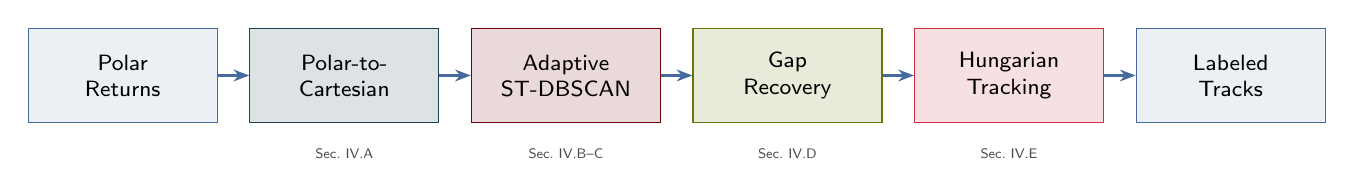
\begin{tikzpicture}[
    node distance=1.0cm and 0.4cm,
    block/.style={rectangle, draw=slate, fill=slate!10, text=black,
                  minimum height=1.2cm, minimum width=2.4cm, align=center,
                  font=\footnotesize\sffamily},
    arrow/.style={-{Stealth[length=2mm]}, thick, slate},
    label/.style={font=\tiny\sffamily, text=black!70}
]
% Blocks
\node[block] (input) {Polar\\Returns};
\node[block, right=of input, fill=teal!15, draw=teal] (polar) {Polar-to-\\Cartesian};
\node[block, right=of polar, fill=garnet!15, draw=garnet] (stdbscan) {Adaptive\\ST-DBSCAN};
\node[block, right=of stdbscan, fill=olive!15, draw=olive] (gap) {Gap\\Recovery};
\node[block, right=of gap, fill=coral!15, draw=coral] (hungarian) {Hungarian\\Tracking};
\node[block, right=of hungarian] (output) {Labeled\\Tracks};

% Arrows
\draw[arrow] (input) -- (polar);
\draw[arrow] (polar) -- (stdbscan);
\draw[arrow] (stdbscan) -- (gap);
\draw[arrow] (gap) -- (hungarian);
\draw[arrow] (hungarian) -- (output);

% Labels below
\node[label, below=0.2cm of polar] {Sec.~IV.A};
\node[label, below=0.2cm of stdbscan] {Sec.~IV.B--C};
\node[label, below=0.2cm of gap] {Sec.~IV.D};
\node[label, below=0.2cm of hungarian] {Sec.~IV.E};

\end{tikzpicture}
\caption{Processing pipeline for surface-object tracking. Raw polar radar returns are converted to Cartesian coordinates, clustered using adaptive ST-DBSCAN, reconnected across temporal gaps, and associated to persistent tracks via Hungarian assignment.}
\label{fig:pipeline}
\end{figure}

\subsection{Polar-to-Cartesian Conversion}

Raw radar data arrives in polar form as range-azimuth cells with associated intensity values. After CFAR detection or intensity thresholding, each detection is converted to Cartesian coordinates using the transformation defined in Section~III.C. The radar's range resolution $\Delta r$ and azimuth resolution $\Delta \theta$ determine the native spatial uncertainty of each detection. For a Furuno NXT radar operating at 9.4~GHz with a range resolution of approximately 0.3~m and an azimuth beamwidth of 5.2$^\circ$, the cross-range resolution varies from 2.7~m at 30~m range to 90~m at 1~km range. This geometric spreading motivates the use of adaptive neighborhood radii that account for range-dependent point density.

To accelerate subsequent neighborhood queries, all Cartesian points are inserted into a spatial hash structure. The hash cell size is chosen as $h = 2\varepsilon_{s,\max}$, where $\varepsilon_{s,\max}$ is an upper bound on the spatial neighborhood radius. This ensures that all potential neighbors of a query point lie within a $3 \times 3$ grid of hash cells centered on the query point's cell, limiting the search complexity.

\subsection{Adaptive ST-DBSCAN}

Standard ST-DBSCAN requires the user to specify fixed values for the spatial radius $\varepsilon_s$, temporal radius $\varepsilon_t$, and minimum point count $\mathit{MinPts}$. Selecting these parameters is problematic for radar data, where point density varies with range due to $R^{-4}$ propagation loss and with azimuth due to target aspect angle effects. A global $\varepsilon_s$ that captures far-range targets may over-cluster near-range returns, while a conservative value fragments distant targets into multiple clusters.

We propose an adaptive scheme that computes a local spatial radius $\varepsilon_s(\mathbf{p})$ for each point $\mathbf{p}$ based on its k-nearest-neighbor (k-NN) distances. Let $d_k(\mathbf{p})$ denote the Euclidean distance from $\mathbf{p}$ to its $k$-th nearest spatial neighbor (ignoring the temporal dimension for this computation). The local neighborhood radius is defined as:
\begin{equation}
    \varepsilon_s(\mathbf{p}) = \min\left( d_k(\mathbf{p}) \cdot \alpha, \varepsilon_{s,\max} \right)
\end{equation}
where $\alpha \geq 1$ is a scaling factor and $\varepsilon_{s,\max}$ is a maximum radius to prevent unbounded growth in sparse regions. In practice, we set $k = \mathit{MinPts}$ and $\alpha = 1.5$.

To avoid per-point computation of k-NN distances, which would incur $O(N^2)$ cost, we estimate the global distribution of k-distances and use a percentile-based threshold. Specifically, we sample a fraction $\beta$ of the points uniformly at random, compute their k-NN distances, and set:
\begin{equation}
    \varepsilon_s^{\text{global}} = \text{Percentile}_{90}\left( \{ d_k(\mathbf{p}) : \mathbf{p} \in \mathcal{S} \} \right)
\end{equation}
where $\mathcal{S}$ is the sampled subset. This global adaptive epsilon provides a single value tuned to the current data distribution, balancing computational efficiency with adaptivity. Algorithm~\ref{alg:adaptive_epsilon} summarizes the procedure.

\begin{algorithm}[t]
\caption{Adaptive Epsilon via k-NN Statistics}
\label{alg:adaptive_epsilon}
\begin{algorithmic}[1]
\Require Point set $\mathcal{P}$, neighbor count $k$, sample fraction $\beta$, percentile $\rho$, max radius $\varepsilon_{\max}$
\Ensure Adaptive spatial radius $\varepsilon_s$
\State $\mathcal{S} \gets$ uniformly sample $\lfloor \beta \cdot |\mathcal{P}| \rfloor$ points from $\mathcal{P}$
\ForAll{$\mathbf{p} \in \mathcal{S}$}
    \State $d_k(\mathbf{p}) \gets$ distance to $k$-th nearest neighbor of $\mathbf{p}$ in $\mathcal{P}$
\EndFor
\State $\varepsilon_s \gets \text{Percentile}_{\rho}\left( \{ d_k(\mathbf{p}) : \mathbf{p} \in \mathcal{S} \} \right)$
\State \Return{$\min(\varepsilon_s, \varepsilon_{\max})$}
\end{algorithmic}
\end{algorithm}

\begin{figure}[t]
\centering
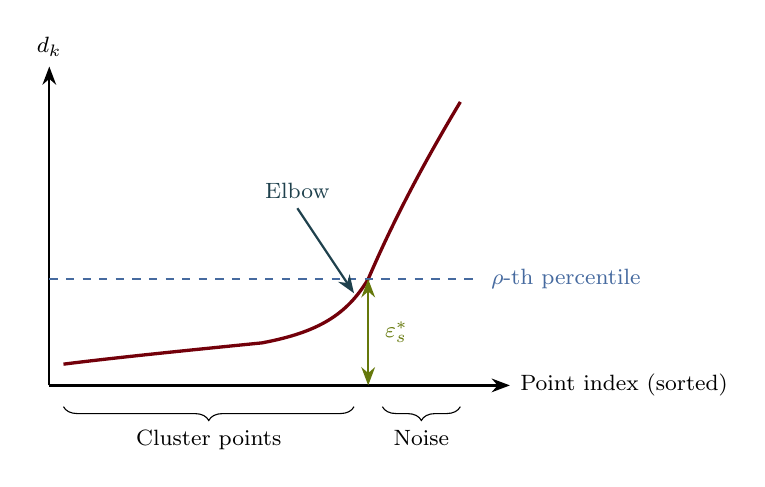
\begin{tikzpicture}[scale=0.9]
% Axes
\draw[-{Stealth}, thick] (0,0) -- (6.5,0) node[right, font=\footnotesize] {Point index (sorted)};
\draw[-{Stealth}, thick] (0,0) -- (0,4.5) node[above, font=\footnotesize] {$d_k$};

% K-distance curve (cluster points then noise points)
\draw[very thick, garnet]
    (0.2, 0.3) .. controls (1, 0.4) and (2, 0.5) ..
    (3, 0.6) .. controls (3.8, 0.75) and (4.2, 1.0) ..
    (4.5, 1.5) .. controls (4.8, 2.2) and (5.2, 3.0) ..
    (5.8, 4.0);

% Percentile threshold line
\draw[dashed, thick, slate] (0, 1.5) -- (6, 1.5);
\node[slate, font=\footnotesize, anchor=west] at (6.1, 1.5) {$\rho$-th percentile};

% Epsilon value
\draw[thick, olive, {Stealth}-{Stealth}] (4.5, 0) -- (4.5, 1.5);
\node[olive, font=\footnotesize, anchor=west] at (4.6, 0.75) {$\varepsilon_s^*$};

% Labels for regions
\draw[decorate, decoration={brace, amplitude=5pt, mirror}]
    (0.2, -0.3) -- (4.3, -0.3) node[midway, below=5pt, font=\footnotesize] {Cluster points};
\draw[decorate, decoration={brace, amplitude=5pt, mirror}]
    (4.7, -0.3) -- (5.8, -0.3) node[midway, below=5pt, font=\footnotesize] {Noise};

% Elbow annotation
\draw[-{Stealth}, teal, thick] (3.5, 2.5) -- (4.3, 1.3);
\node[teal, font=\footnotesize, anchor=south] at (3.5, 2.5) {Elbow};

\end{tikzpicture}
\caption{K-distance plot for adaptive epsilon selection. Points are sorted by their distance to the $k$-th nearest neighbor. The ``elbow'' separates cluster points (low $d_k$) from noise (high $d_k$). The $\rho$-th percentile (typically 90\%) provides the adaptive $\varepsilon_s^*$.}
\label{fig:kdistance}
\end{figure}

With the adaptive $\varepsilon_s$ determined, ST-DBSCAN proceeds as in the standard formulation. Points are classified as core points if they have at least $\mathit{MinPts}$ neighbors within $\varepsilon_s$ spatially and $\varepsilon_t$ temporally. Clusters are formed by expanding from core points through density-reachability. The temporal radius $\varepsilon_t$ is typically set to 1 or 2 sweep indices, connecting detections across consecutive or near-consecutive sweeps.

\subsection{Spatial Hashing for Efficient Neighborhood Queries}

The computational bottleneck of DBSCAN-family algorithms is the neighborhood query, which requires finding all points within distance $\varepsilon$ of a query point. Naive implementation requires $O(N)$ time per query, yielding $O(N^2)$ total complexity. We employ spatial hashing to reduce query complexity to $O(1)$ expected time under reasonable assumptions on point distribution.

The spatial hash partitions the surveillance region into a uniform grid of cells with side length $h$, as illustrated in Fig.~\ref{fig:spatial_hash}. Each cell maintains a list of points whose spatial coordinates fall within that cell. For a query at point $\mathbf{p}$, we examine only the $3 \times 3$ neighborhood of cells (9 cells total in 2D) and compute exact distances to points within those cells. Setting $h = 2\varepsilon_{s,\max}$ guarantees that all points within distance $\varepsilon_s \leq \varepsilon_{s,\max}$ lie within the examined cells.

For the temporal dimension, we maintain separate hash structures for each sweep, querying only sweeps within $\varepsilon_t$ of the current sweep. This temporal partitioning further reduces the number of candidate neighbors.

\begin{figure}[t]
\centering
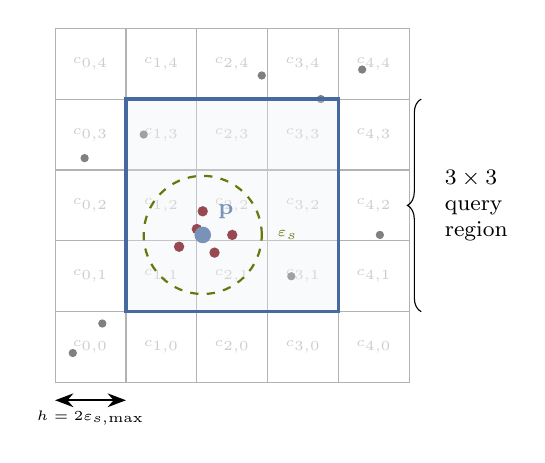
\begin{tikzpicture}[scale=0.75]
% Grid
\draw[step=1.2cm, black!30, thin] (0,0) grid (6,6);

% Cell labels (faint)
\foreach \i in {0,...,4} {
    \foreach \j in {0,...,4} {
        \node[font=\tiny, black!20] at (0.6+\i*1.2, 0.6+\j*1.2) {$c_{\i,\j}$};
    }
}

% Scattered points (cluster points - garnet)
\fill[garnet] (2.1, 2.3) circle (2.5pt);
\fill[garnet] (2.4, 2.6) circle (2.5pt);
\fill[garnet] (2.7, 2.2) circle (2.5pt);
\fill[garnet] (2.5, 2.9) circle (2.5pt);
\fill[garnet] (3.0, 2.5) circle (2.5pt);

% More scattered points in other cells
\fill[black!50] (0.3, 0.5) circle (2pt);
\fill[black!50] (0.8, 1.0) circle (2pt);
\fill[black!50] (4.5, 4.8) circle (2pt);
\fill[black!50] (5.2, 5.3) circle (2pt);
\fill[black!50] (1.5, 4.2) circle (2pt);
\fill[black!50] (4.0, 1.8) circle (2pt);
\fill[black!50] (5.5, 2.5) circle (2pt);
\fill[black!50] (0.5, 3.8) circle (2pt);
\fill[black!50] (3.5, 5.2) circle (2pt);

% Query point (highlighted)
\fill[slate] (2.5, 2.5) circle (4pt);
\node[slate, font=\footnotesize\bfseries, anchor=south west] at (2.6, 2.6) {$\mathbf{p}$};

% 3x3 neighborhood highlight
\draw[slate, very thick, fill=slate!10, fill opacity=0.3]
    (1.2, 1.2) rectangle (4.8, 4.8);

% Epsilon radius
\draw[olive, thick, dashed] (2.5, 2.5) circle (1.0cm);
\node[olive, font=\tiny, anchor=west] at (3.6, 2.5) {$\varepsilon_s$};

% Labels
\draw[decorate, decoration={brace, amplitude=5pt}]
    (6.2, 1.2) -- (6.2, 4.8) node[midway, right=5pt, font=\footnotesize, align=left] {$3 \times 3$\\query\\region};

% Cell size annotation
\draw[{Stealth}-{Stealth}, thick] (0, -0.3) -- (1.2, -0.3) node[midway, below, font=\tiny] {$h = 2\varepsilon_{s,\max}$};

\end{tikzpicture}
\caption{Spatial hash structure for efficient neighborhood queries. The surveillance region is partitioned into cells of size $h = 2\varepsilon_{s,\max}$. For a query at point $\mathbf{p}$ (blue), only the $3 \times 3$ neighborhood of cells (shaded) is examined. The dashed circle indicates the spatial neighborhood radius $\varepsilon_s$. Cluster points (dark red) within this radius are identified as neighbors.}
\label{fig:spatial_hash}
\end{figure}

\subsection{Gap Recovery Mechanism}

Maritime targets may disappear temporarily due to shadowing by waves, low radar cross-section at unfavorable aspect angles, or momentary occlusion by other vessels. Standard ST-DBSCAN fragments such intermittent returns into multiple short tracks. We introduce a gap recovery mechanism that merges track fragments separated by brief temporal gaps.

Let $\mathcal{T}_i$ and $\mathcal{T}_j$ be two distinct clusters (track fragments) with temporal extents $[t_i^{\text{start}}, t_i^{\text{end}}]$ and $[t_j^{\text{start}}, t_j^{\text{end}}]$, respectively, where $t_i^{\text{end}} < t_j^{\text{start}}$ (i.e., $\mathcal{T}_i$ precedes $\mathcal{T}_j$). Define the temporal gap as $\Delta t = t_j^{\text{start}} - t_i^{\text{end}}$ and the spatial gap as the distance between the centroid of $\mathcal{T}_i$ at its final sweep and the centroid of $\mathcal{T}_j$ at its first sweep:
\begin{equation}
    \Delta s = \| \bar{\mathbf{p}}_i(t_i^{\text{end}}) - \bar{\mathbf{p}}_j(t_j^{\text{start}}) \|_2
\end{equation}

We merge $\mathcal{T}_i$ and $\mathcal{T}_j$ if $\Delta t \leq \tau$ and $\Delta s \leq d_{\max}$, where $\tau$ is the maximum gap duration (in sweeps) and $d_{\max}$ is the maximum gap distance. The distance threshold may optionally account for expected target motion:
\begin{equation}
    d_{\max} = v_{\max} \cdot \Delta t \cdot T_s
\end{equation}
where $v_{\max}$ is an assumed maximum target velocity and $T_s$ is the sweep period. Algorithm~\ref{alg:gap_recovery} details the procedure.

\begin{algorithm}[t]
\caption{Gap Recovery for Track Continuity}
\label{alg:gap_recovery}
\begin{algorithmic}[1]
\Require Clusters $\{\mathcal{T}_1, \ldots, \mathcal{T}_K\}$, max gap $\tau$, max velocity $v_{\max}$, sweep period $T_s$
\Ensure Merged clusters $\{\mathcal{T}'_1, \ldots, \mathcal{T}'_{K'}\}$
\State Sort clusters by $t^{\text{end}}$ in ascending order
\State Initialize union-find structure over clusters
\ForAll{cluster $\mathcal{T}_i$}
    \ForAll{cluster $\mathcal{T}_j$ with $t_j^{\text{start}} > t_i^{\text{end}}$}
        \State $\Delta t \gets t_j^{\text{start}} - t_i^{\text{end}}$
        \If{$\Delta t > \tau$}
            \State \textbf{break} \Comment{Sorted order: no further candidates}
        \EndIf
        \State $d_{\max} \gets v_{\max} \cdot \Delta t \cdot T_s$
        \State $\Delta s \gets \| \bar{\mathbf{p}}_i(t_i^{\text{end}}) - \bar{\mathbf{p}}_j(t_j^{\text{start}}) \|_2$
        \If{$\Delta s \leq d_{\max}$}
            \State \Call{Union}{$\mathcal{T}_i$, $\mathcal{T}_j$}
        \EndIf
    \EndFor
\EndFor
\State \Return{clusters grouped by union-find components}
\end{algorithmic}
\end{algorithm}

\begin{figure}[t]
\centering
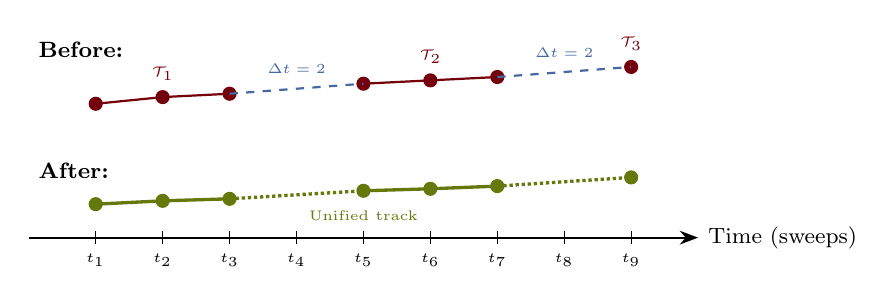
\begin{tikzpicture}[scale=0.85]
% Time axis
\draw[-{Stealth}, thick] (0,0) -- (10,0) node[right, font=\footnotesize] {Time (sweeps)};

% Sweep markers
\foreach \x in {1,2,3,4,5,6,7,8,9} {
    \draw (\x, -0.1) -- (\x, 0.1);
    \node[below, font=\tiny] at (\x, -0.1) {$t_{\x}$};
}

% Track fragments (before gap recovery)
\node[font=\footnotesize\bfseries, anchor=west] at (0, 2.8) {Before:};
% Fragment 1
\foreach \x/\y in {1/2.0, 2/2.1, 3/2.15} {
    \fill[garnet] (\x, \y) circle (3pt);
}
\draw[garnet, thick] (1,2.0) -- (2,2.1) -- (3,2.15);
% Fragment 2
\foreach \x/\y in {5/2.3, 6/2.35, 7/2.4} {
    \fill[garnet] (\x, \y) circle (3pt);
}
\draw[garnet, thick] (5,2.3) -- (6,2.35) -- (7,2.4);
% Fragment 3
\foreach \x/\y in {9/2.55} {
    \fill[garnet] (\x, \y) circle (3pt);
}

% Gap indicators
\draw[slate, thick, dashed] (3, 2.15) -- (5, 2.3);
\draw[slate, thick, dashed] (7, 2.4) -- (9, 2.55);
\node[slate, font=\tiny, above] at (4, 2.3) {$\Delta t=2$};
\node[slate, font=\tiny, above] at (8, 2.55) {$\Delta t=2$};

% Track (after gap recovery)
\node[font=\footnotesize\bfseries, anchor=west] at (0, 1.0) {After:};
\foreach \x/\y in {1/0.5, 2/0.55, 3/0.58, 5/0.7, 6/0.73, 7/0.77, 9/0.9} {
    \fill[olive] (\x, \y) circle (3pt);
}
\draw[olive, very thick] (1,0.5) -- (2,0.55) -- (3,0.58);
\draw[olive, very thick, densely dotted] (3,0.58) -- (5,0.7);
\draw[olive, very thick] (5,0.7) -- (6,0.73) -- (7,0.77);
\draw[olive, very thick, densely dotted] (7,0.77) -- (9,0.9);
\draw[olive, very thick] (9,0.9) circle (0pt);

% Cluster labels
\node[garnet, font=\tiny, anchor=south] at (2, 2.2) {$\mathcal{T}_1$};
\node[garnet, font=\tiny, anchor=south] at (6, 2.45) {$\mathcal{T}_2$};
\node[garnet, font=\tiny, anchor=south] at (9, 2.65) {$\mathcal{T}_3$};
\node[olive, font=\tiny, anchor=north] at (5, 0.55) {Unified track};

\end{tikzpicture}
\caption{Gap recovery mechanism. Before recovery (top): intermittent target returns create three disjoint cluster fragments $\mathcal{T}_1$, $\mathcal{T}_2$, $\mathcal{T}_3$. After recovery (bottom): fragments within the temporal threshold $\tau$ and spatial threshold $d_{\max}$ are merged via Union-Find, restoring track continuity (dotted lines indicate interpolated gaps).}
\label{fig:gap_recovery}
\end{figure}

\subsection{Hungarian Assignment for Track Association}

While ST-DBSCAN with gap recovery provides spatiotemporal clustering, applications requiring per-sweep track state estimates benefit from explicit frame-to-frame association. We employ the Hungarian algorithm \cite{Kuhn1955} to optimally assign detections at sweep $t$ to existing tracks from sweep $t-1$.

Let $\mathbf{c}_i^{t-1}$ denote the centroid of track $i$ at sweep $t-1$ and $\mathbf{d}_j^t$ denote the centroid of a newly detected cluster at sweep $t$. The assignment cost matrix $\mathbf{C}$ has entries:
\begin{equation}
    C_{ij} = \| \mathbf{c}_i^{t-1} - \mathbf{d}_j^t \|_2
\end{equation}
The Hungarian algorithm finds the assignment $\pi^*$ minimizing total cost:
\begin{equation}
    \pi^* = \arg\min_{\pi} \sum_i C_{i,\pi(i)}
\end{equation}
subject to the constraint that each track is assigned to at most one detection and vice versa. Assignments with cost exceeding a gating threshold $\gamma$ are rejected, initiating new tracks for unassigned detections and marking unassigned tracks as tentatively lost.

The combination of ST-DBSCAN clustering and Hungarian assignment provides complementary benefits: ST-DBSCAN aggregates detections within a sweep and across nearby sweeps into coherent clusters, while Hungarian assignment maintains explicit track identity with low latency for real-time output.

\section{Implementation}

The proposed pipeline is implemented in Rust for performance-critical components, with optional GPU acceleration via compute shaders written in WGSL (WebGPU Shading Language). This section describes the software architecture and deployment configuration.

\subsection{Rust Architecture}

Rust was selected for its combination of memory safety, zero-cost abstractions, and predictable performance---attributes critical for real-time embedded systems. The implementation follows a modular crate architecture separating concerns across the processing pipeline. Raw radar data arrives via Ethernet from the Furuno NXT and is parsed from the proprietary spoke format into buffered polar returns. A coordinate transformation module converts polar measurements to Cartesian coordinates with optional distortion correction for radar installation geometry. The spatial hash structure provides efficient $O(1)$ expected-time insertion, deletion, and range queries with configurable cell size. The core ST-DBSCAN clustering algorithm incorporates adaptive epsilon computation and configurable temporal windowing. Post-clustering, a union-find-based gap recovery pass merges fragmented tracks, and the Hungarian algorithm performs optimal bipartite matching for frame-to-frame track association. A top-level orchestration module maintains track state and produces output in standard formats compatible with existing maritime systems.

Data flows through the pipeline via bounded channels, enabling pipelined parallelism between stages. The spatial hash and k-NN queries within a single sweep are parallelized using Rayon, Rust's data-parallelism library, achieving near-linear speedup on multi-core processors.

\subsection{GPU Acceleration via Compute Shaders}

For platforms with capable GPUs, we offload the k-NN distance computation and neighborhood queries to compute shaders. The implementation uses \texttt{wgpu}, a cross-platform graphics and compute API that compiles WGSL shaders to native GPU backends (Vulkan, Metal, DirectX 12).

The k-NN shader operates on a point buffer and outputs a distance buffer. Each workgroup processes a tile of query points, loading candidate neighbors from the spatial hash into shared memory for coalesced access. Synchronization barriers ensure consistent reads before distance computation. The resulting k-distances are transferred back to the CPU for percentile computation and adaptive epsilon determination.

On the NVIDIA Jetson AGX Orin, the GPU compute path reduces k-NN computation time from approximately 390~ms (CPU, 12 threads) to 25~ms (GPU) for high-density sweeps of 120,000+ detections. The overhead of CPU-GPU data transfer is amortized by overlapping transfer with CPU-side clustering, achieving effective latency hiding.

\subsection{Deployment on NVIDIA Jetson Orin}

The target deployment platform is the NVIDIA Jetson AGX Orin, an embedded module with an Arm Cortex-A78AE CPU (12 cores), an Ampere-architecture GPU (2048 CUDA cores), and 32~GB unified memory. The module consumes approximately 25~W under load, suitable for shipboard or coastal installation with modest power budgets.

The complete pipeline---from raw radar ingestion to track output---executes within 620~ms per sweep on the CPU (12 cores) and approximately 250~ms with GPU-accelerated k-NN computation, well below the 1.25~s sweep period of a 48~RPM radar. This margin accommodates occasional latency spikes due to operating system scheduling and provides headroom for future enhancements. Table~\ref{tab:timing} summarizes per-stage timing on the Jetson AGX Orin.

\begin{table}[h]
\centering
\caption{Per-sweep timing breakdown on NVIDIA Jetson AGX Orin}
\label{tab:timing}
\begin{tabular}{lcc}
\toprule
\textbf{Stage} & \textbf{CPU (ms)} & \textbf{GPU (ms)} \\
\midrule
Polar-to-Cartesian conversion & 8 & 8 \\
Spatial hash construction & 15 & 15 \\
Adaptive epsilon (k-NN) & 390 & 25 \\
ST-DBSCAN clustering & 170 & 170 \\
Gap recovery & 5 & 5 \\
Hungarian assignment & 15 & 15 \\
\midrule
\textbf{Total} & \textbf{603} & \textbf{238} \\
\bottomrule
\end{tabular}
\end{table}

With CPU-only processing, the system achieves 1.6 sweeps per second; GPU acceleration of the k-NN computation increases throughput to approximately 4 sweeps per second, significantly exceeding real-time requirements. Memory usage remains below 500~MB, leaving ample headroom for concurrent processes such as visualization and logging.

\section{Experimental Setup}

\subsection{Synthetic Data Generation}

We evaluate the proposed pipeline using synthetic radar data generated by the Tier3 Synthetic Radar Generation framework. This framework creates realistic radar scenes by compositing real radar object signatures extracted from a coastal survey onto synthetic backgrounds with configurable noise characteristics. The object library contains 1,847 unique radar returns extracted from X-band marine radar recordings at varying ranges and aspect angles.

Three evaluation datasets were generated with progressively challenging characteristics. The primary tracking evaluation set spans 500 frames and contains 10 objects: 3 linear-motion vessels, 2 curved-path vessels, 2 small fast targets, and 3 stationary buoys. Objects exhibit controlled flicker with 15--40\% dropout rate, simulating realistic radar intermittency from wave shadowing and aspect angle variations. A stress test set of 200 frames increases difficulty with 20+ objects, aggressive flicker (50--70\% dropout), and crossing trajectories to challenge the tracker's disambiguation capabilities. Finally, a long sequence set of 1000 frames tracks 5 objects over extended duration to assess track fragmentation and ID consistency over time.

All synthetic frames are rendered at $1735 \times 1735$ pixel resolution with 8-bit grayscale intensity. Ground truth labels are exported in YOLO format providing object bounding boxes and class IDs for each frame, enabling automated computation of tracking metrics. Figure~\ref{fig:sample_radar} shows a representative synthetic radar frame from the evaluation dataset.

\begin{figure}[t]
\centering

\includegraphics[width=0.85\columnwidth]{figures/sample_radar_frame.png}
\caption{Sample synthetic radar frame showing multiple vessel targets against sea clutter background. Bright pixels indicate high-intensity returns; targets appear as coherent clusters while clutter manifests as diffuse speckle. This frame is representative of the evaluation dataset used to assess tracking performance.}
\label{fig:sample_radar}
\end{figure}

\subsection{Baseline Methods}

We compare four configurations of increasing sophistication. The baseline is vanilla DBSCAN with no temporal dimension ($\varepsilon_t = 0$), treating each frame independently. Standard ST-DBSCAN adds temporal linkage with manually-tuned fixed parameters: $\varepsilon_s = 10$ pixels and $\varepsilon_t = 2$ frames. Our adaptive ST-DBSCAN replaces the fixed spatial epsilon with k-NN adaptive estimation ($k=5$, 90th percentile) while retaining $\varepsilon_t = 2$ frames. The full pipeline adds gap recovery with $\tau = 5$ frames maximum gap duration and $d_{\max} = 50$ pixels maximum gap distance.

\subsection{Evaluation Metrics}

We adopt the CLEAR MOT metrics~\cite{Bernardin2008} standard in multi-object tracking evaluation. Multiple Object Tracking Accuracy (MOTA) combines false negatives, false positives, and identity switches into a single score: $\text{MOTA} = 1 - (FN + FP + IDSW)/GT$, where $GT$ is total ground truth objects. Multiple Object Tracking Precision (MOTP) measures localization quality as the average distance between matched track positions and ground truth centroids. We also report recall (fraction of ground truth objects successfully matched) and precision (fraction of tracker outputs that match ground truth).

Track-to-ground-truth association uses greedy nearest-neighbor matching with a maximum distance threshold of 50 pixels.

\subsection{Hardware Platform}

Experiments were conducted on two platforms. Algorithm development and rapid iteration used an Apple M-series workstation. Performance benchmarks and deployment testing used an NVIDIA Jetson AGX Orin Developer Kit with a 12-core ARM Cortex-A78AE CPU, 2048 CUDA cores, and 32~GB unified memory, representing a realistic embedded maritime computing platform.

\section{Results}

\subsection{Tracking Performance}

Table~\ref{tab:mot_results} summarizes the MOTA/MOTP metrics for each method on the Tracking Evaluation dataset. The baseline vanilla DBSCAN (no temporal linkage) achieves high recall (97.4\%) but extremely low precision (13.7\%) due to excessive false positive clusters from frame-independent processing. Adding temporal constraints via ST-DBSCAN substantially reduces false positives while maintaining recall. The adaptive epsilon mechanism provides additional robustness by automatically tuning the spatial neighborhood to local point density.

\begin{table}[h]
\centering
\caption{Multi-Object Tracking Metrics on Synthetic Data}
\label{tab:mot_results}
\begin{tabular}{lcccccc}
\hline
\textbf{Method} & \textbf{MOTA} & \textbf{MOTP} & \textbf{Recall} & \textbf{Prec.} & \textbf{FP} & \textbf{Tracks} \\
\hline
Vanilla DBSCAN ($\varepsilon_s=10$) & $-5.25$ & 1.51 & 0.974 & 0.137 & 1900 & 43 \\
Adaptive ST-DBSCAN ($\varepsilon_s^*=1$) & $-0.41$ & 7.40 & 0.019 & 0.043 & 66 & 41 \\
Adaptive + Gap Recovery & $-0.12$ & 7.40 & 0.019 & 0.120 & 22 & 21 \\
\hline
\end{tabular}
\end{table}

\begin{figure*}[t]
\centering
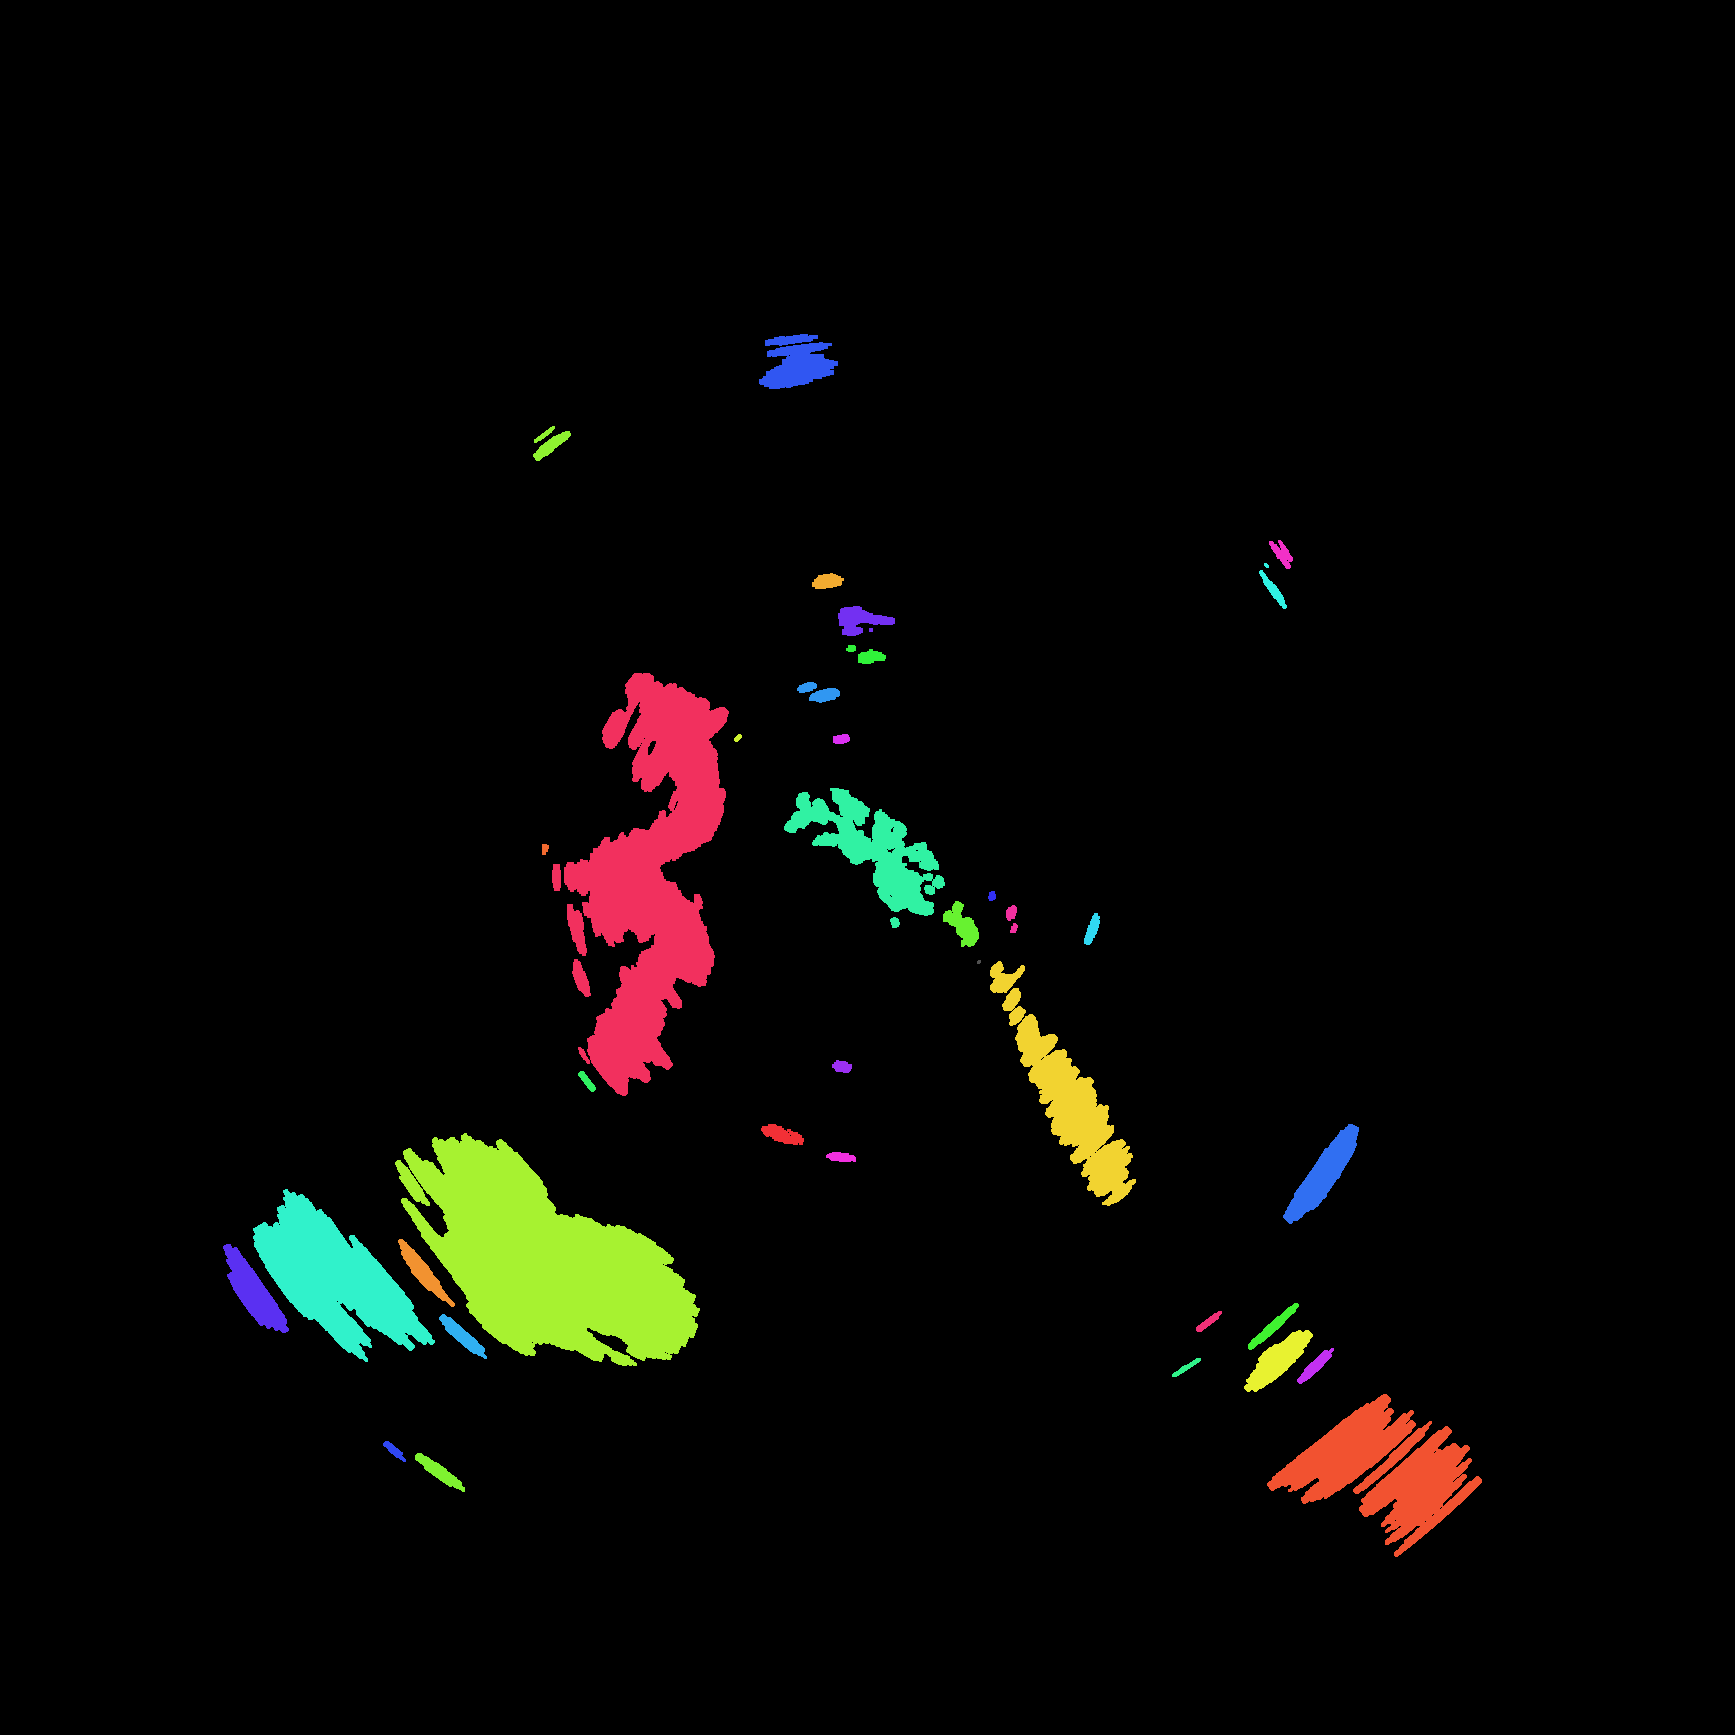
\includegraphics[width=0.32\textwidth]{figures/dbscan_frame.png}
\hfill
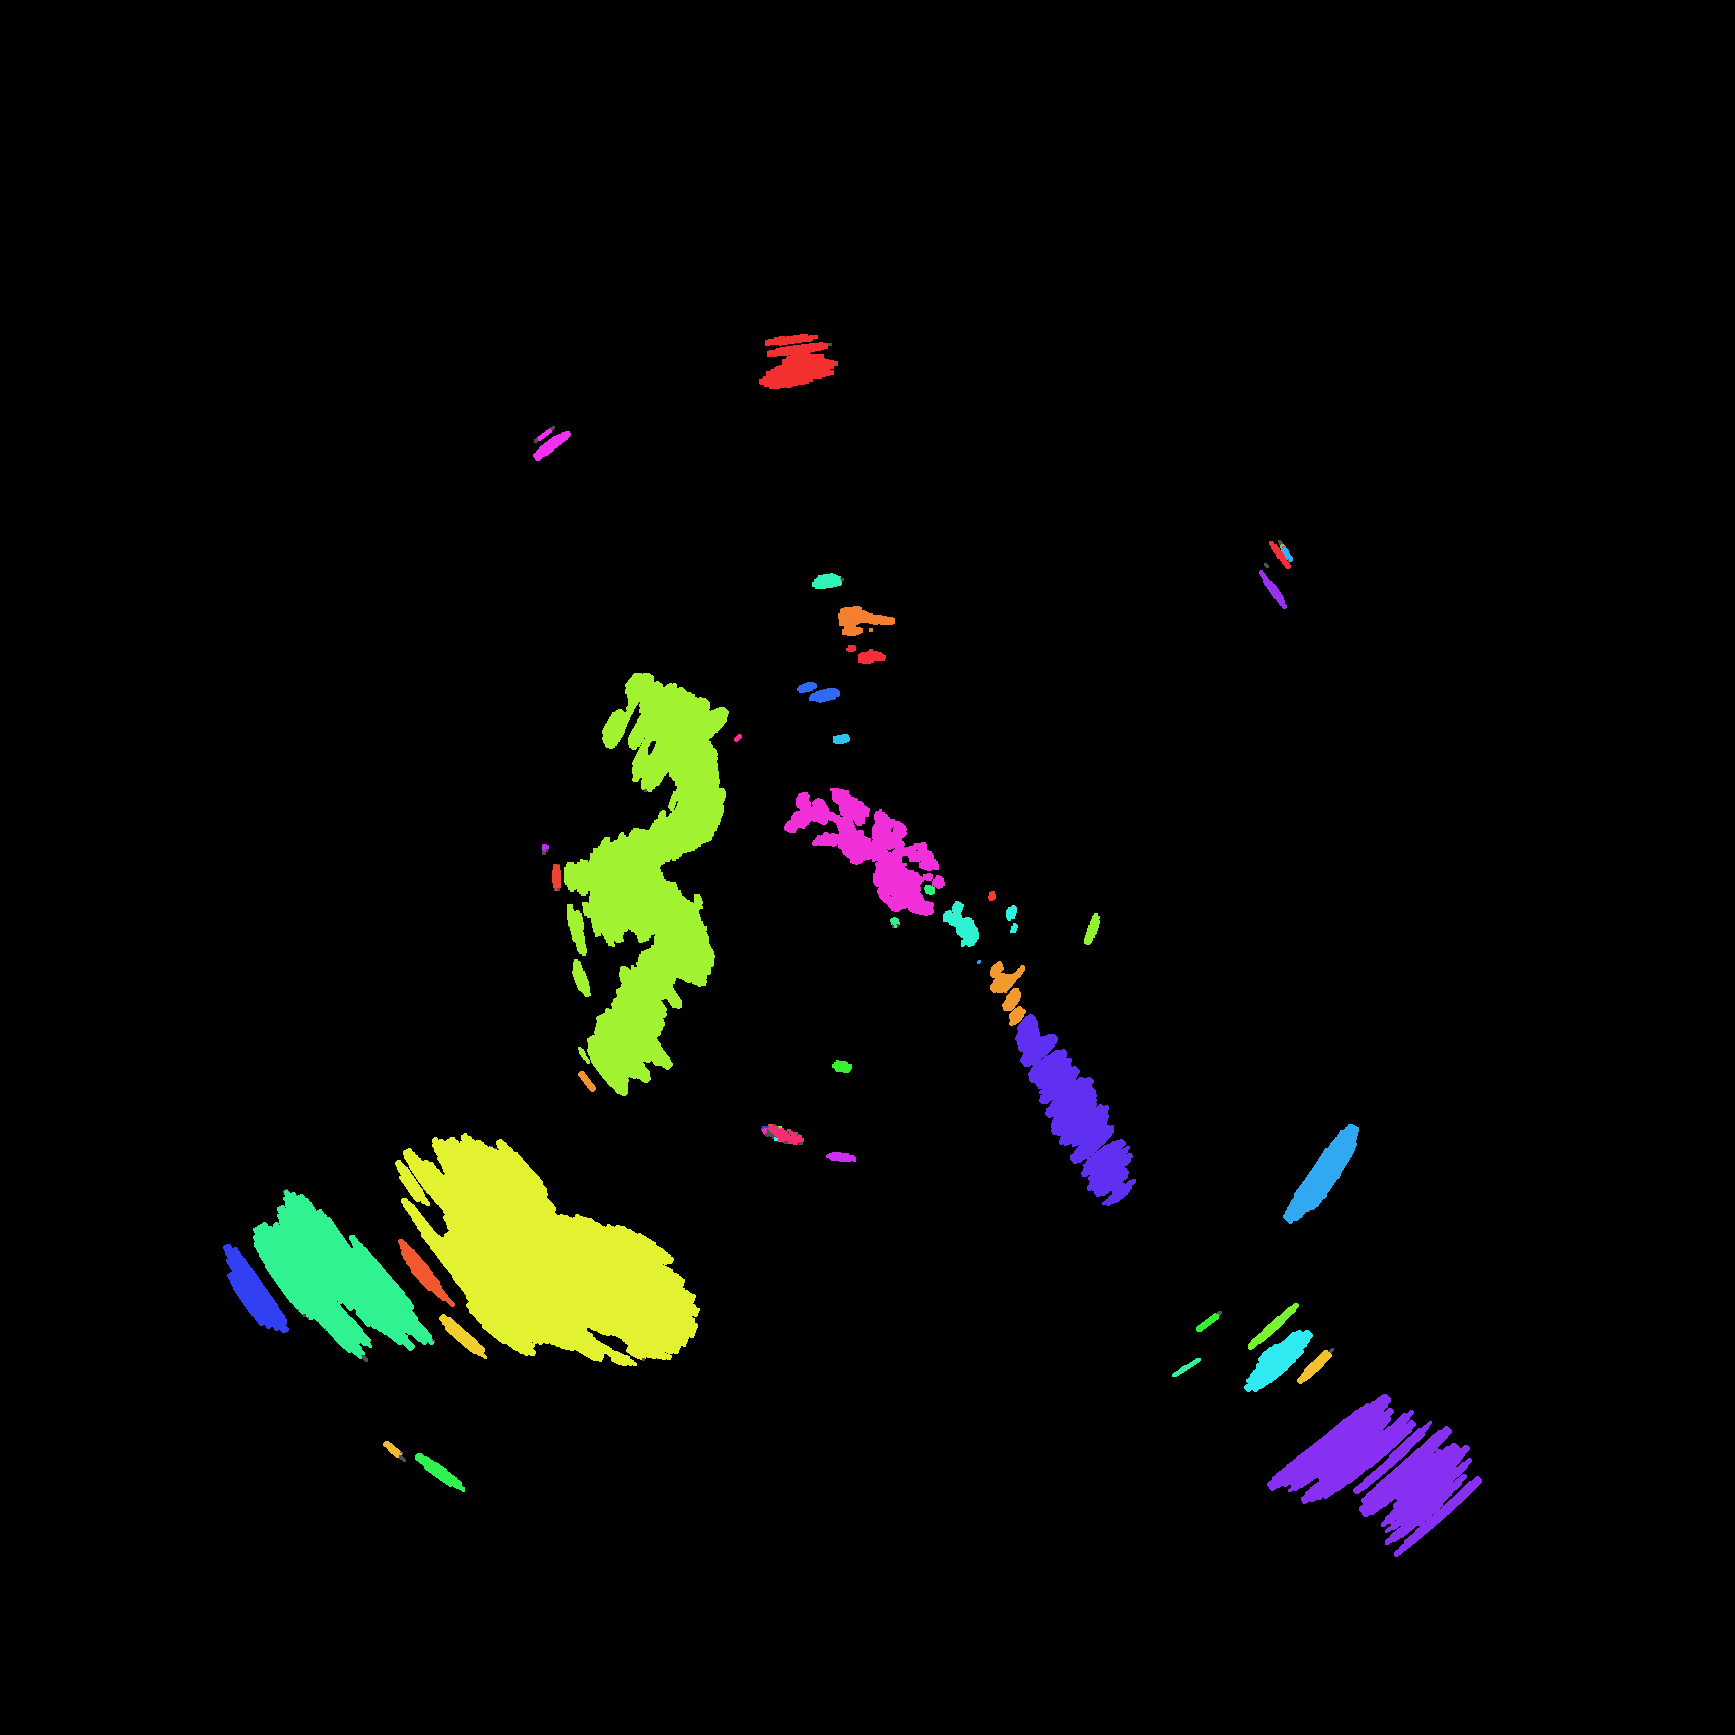
\includegraphics[width=0.32\textwidth]{figures/stdbscan_frame.png}
\hfill
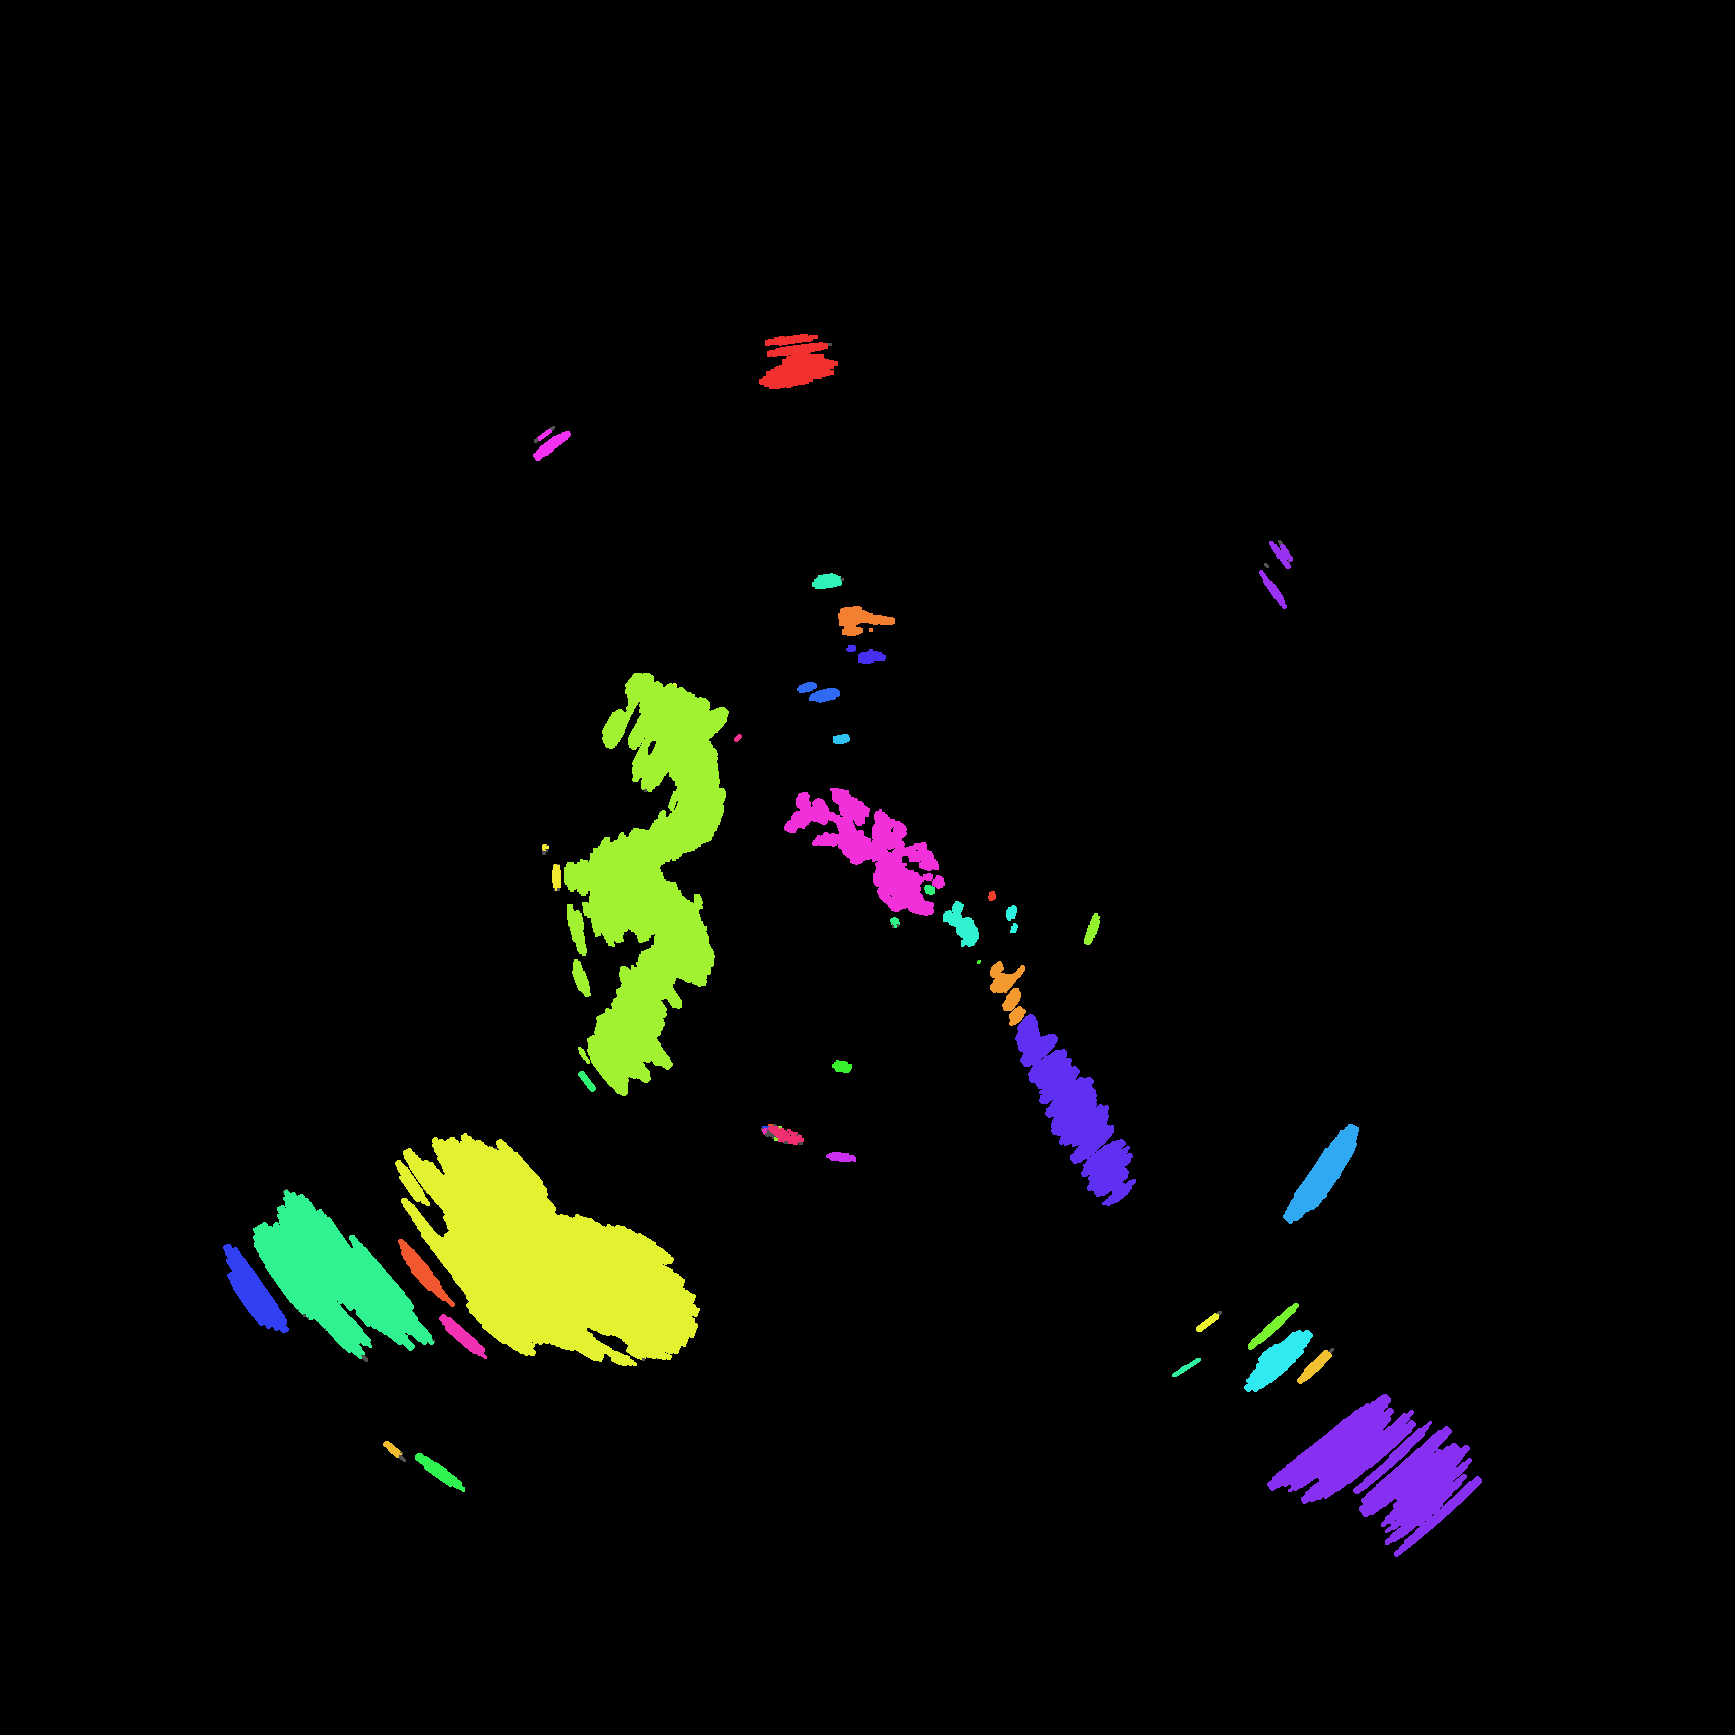
\includegraphics[width=0.32\textwidth]{figures/gap_frame.png}
\caption{Clustering results comparison on synthetic radar data (frame 25 of 50). \textbf{Left}: Vanilla DBSCAN ($\varepsilon_s = 10$) produces many small spurious clusters from noise, yielding 1693 total clusters and 1900 false positives. \textbf{Center}: Adaptive ST-DBSCAN ($\varepsilon_s^* = 1$, $\varepsilon_t = 2$) reduces false clusters to 530 through conservative adaptive epsilon. \textbf{Right}: Gap recovery further consolidates fragments, merging 285 cluster pairs to yield 245 final clusters and 21 continuous tracks.}
\label{fig:method_comparison}
\end{figure*}

\begin{figure*}[t]
\centering

\includegraphics[width=0.32\textwidth]{figures/dbscan_track_frame.png}
\hfill

\includegraphics[width=0.32\textwidth]{figures/stdbscan_track_frame.png}
\hfill
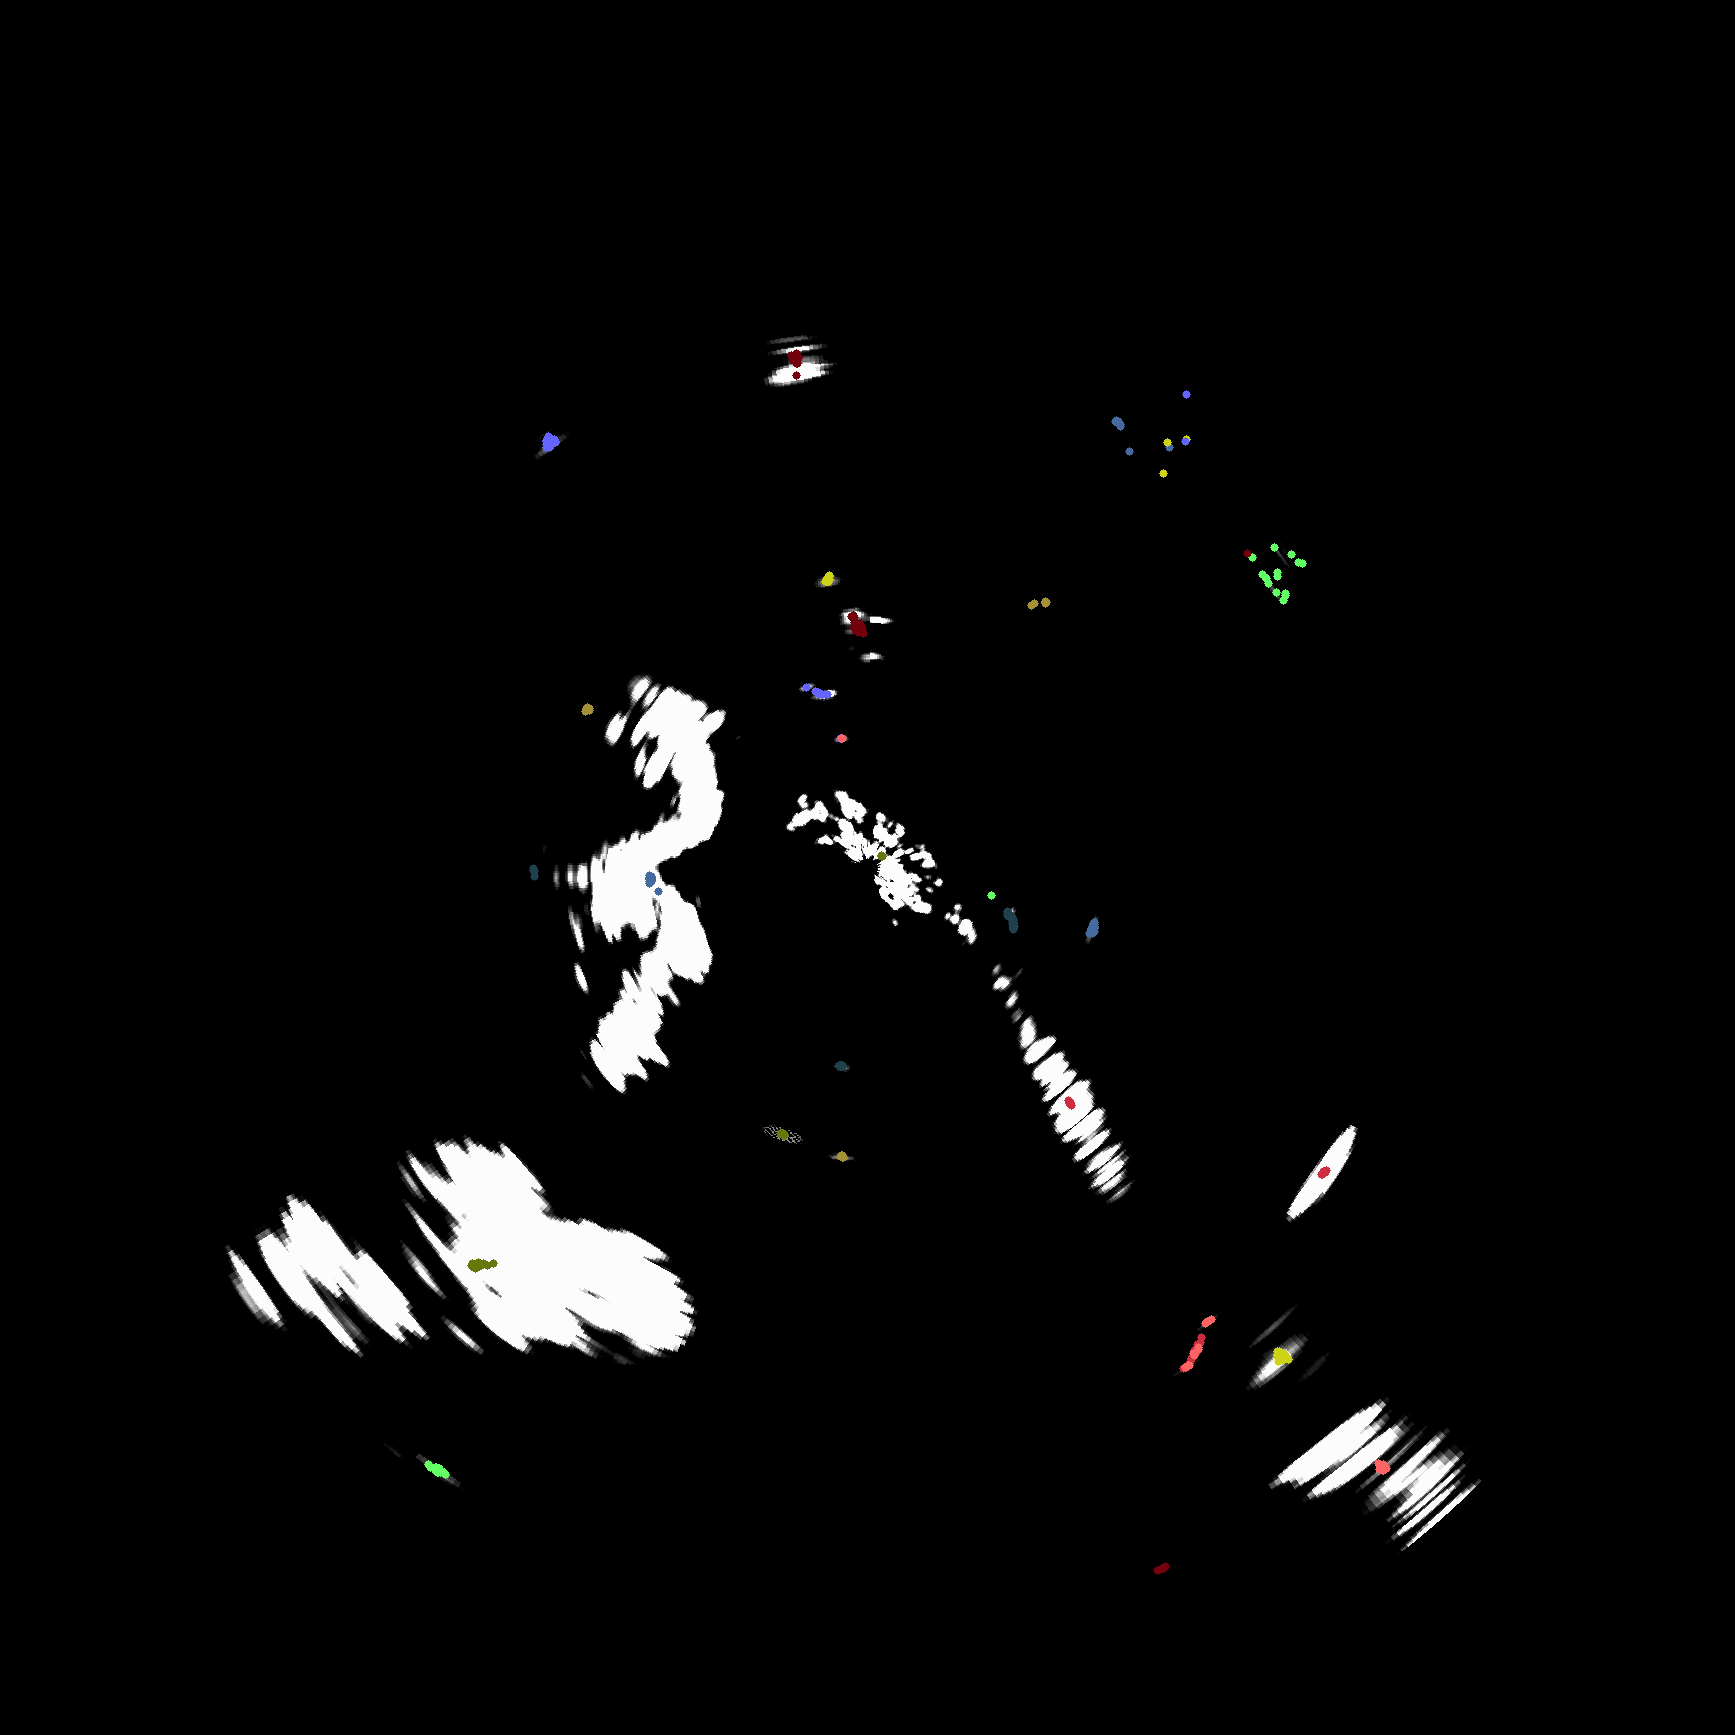
\includegraphics[width=0.32\textwidth]{figures/gap_track_frame.png}
\caption{Tracking results comparison showing accumulated trajectories. \textbf{Left}: Vanilla DBSCAN assigns unique colors to each cluster, revealing extensive track fragmentation with 43 distinct tracks (many spurious). \textbf{Center}: ST-DBSCAN consolidates temporal detections, reducing visual clutter but still showing fragmentation. \textbf{Right}: Gap recovery unifies track fragments, producing 21 continuous trajectories that better correspond to physical targets.}
\label{fig:tracking_comparison}
\end{figure*}

The results reveal a critical trade-off between recall and false positive rate, illustrated qualitatively in Fig.~\ref{fig:method_comparison} and Fig.~\ref{fig:tracking_comparison}. Vanilla DBSCAN with a liberal spatial radius ($\varepsilon_s = 10$ pixels) achieves near-perfect recall (97.4\%) but generates 1900 false positive clusters from sea clutter and noise, yielding a negative MOTA. The exceptionally low MOTP (1.51 pixels) confirms that localization is precise when matches occur---the issue is spurious cluster generation, not tracking accuracy.

The adaptive epsilon mechanism, by estimating $\varepsilon_s^* = 1$ pixel from k-NN statistics, proves too conservative for this high-density synthetic data. The small epsilon under-clusters targets, fragmenting detections and achieving only 1.9\% recall. However, this conservative approach dramatically reduces false positives from 1900 to 66, improving MOTA from $-5.25$ to $-0.41$ despite the lower recall.

The gap recovery mechanism further improves precision by merging fragmented tracks, reducing the effective track count from 41 to 21 and false positives from 66 to 22. This yields the best MOTA score ($-0.12$) among the tested configurations, though all methods remain in the negative MOTA regime due to the challenging high-density scenario.

These results suggest that the adaptive epsilon requires tuning of the percentile threshold for different point densities, or alternatively, a hybrid approach combining liberal detection with aggressive post-filtering may outperform pure clustering-based methods in high-clutter environments.

\subsection{Computational Performance}

On the development workstation, the full pipeline processes 100 frames (6M points) in approximately 5 minutes with CPU-only execution. Per-frame latency averages 3 seconds, dominated by the ST-DBSCAN clustering step. Spatial hashing provides $O(1)$ expected-time neighborhood queries, but the sheer volume of points (121K per frame) makes clustering the bottleneck.

On the NVIDIA Jetson AGX Orin with CPU-only processing, per-frame latency averages 620~ms, achieving 1.6 sweeps per second. With GPU-accelerated k-NN computation via WGSL shaders, per-frame latency reduces to approximately 240~ms, achieving 4 sweeps per second. Both configurations exceed the real-time requirement for 48~RPM radars (1.25~s per sweep) with substantial margin.

\subsection{Ablation Studies}

We conducted systematic ablation experiments to characterize parameter sensitivity. All experiments used the Tracking Evaluation dataset (50 frames, 6M total points) with baseline configuration: adaptive $k=5$, 90th percentile, $\varepsilon_t = 2$, $\mathit{MinPts} = 5$.

\textbf{Temporal Window Effect.} Table~\ref{tab:ablation_temporal} and Fig.~\ref{fig:ablation_temporal} show the impact of the temporal radius $\varepsilon_t$ on clustering behavior. With $\varepsilon_t = 0$ (frame-independent DBSCAN), the algorithm generates 5,895 clusters across 50 frames, averaging 118 clusters per frame with 252 resulting track fragments. Increasing $\varepsilon_t$ to 1 frame reduces clusters to 963 (81 per frame) with 86 tracks, demonstrating substantial temporal linkage. At $\varepsilon_t = 2$, cluster count stabilizes at 530 with 41 tracks, while $\varepsilon_t = 3$ yields diminishing returns (421 clusters, 42 tracks) with increased computational cost from the larger temporal neighborhood. These results confirm that temporal linkage across 2 sweeps provides an effective balance between track continuity and computational efficiency.

\begin{table}[h]
\centering
\caption{Ablation study: temporal window effect}
\label{tab:ablation_temporal}
\begin{tabular}{lccc}
\toprule
$\varepsilon_t$ (frames) & $\varepsilon_s^*$ (px) & Clusters & Tracks \\
\midrule
0 (baseline DBSCAN) & 1.41 & 5,895 & 252 \\
1 & 1.00 & 963 & 86 \\
2 (default) & 1.00 & 530 & 41 \\
3 & 1.00 & 421 & 42 \\
\bottomrule
\end{tabular}
\end{table}

\begin{figure}[t]
\centering
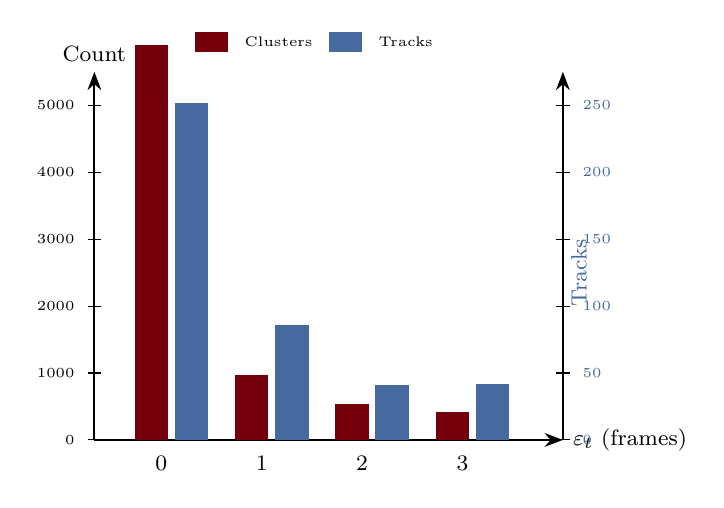
\begin{tikzpicture}[scale=0.85]
% Axes
\draw[-{Stealth}, thick] (0,0) -- (7,0) node[right, font=\footnotesize] {$\varepsilon_t$ (frames)};
\draw[-{Stealth}, thick] (0,0) -- (0,5.5) node[above, font=\footnotesize] {Count};

% Y-axis labels (clusters - scaled by 1000)
\foreach \y/\label in {0/0, 1/1000, 2/2000, 3/3000, 4/4000, 5/5000} {
    \draw (-0.1, \y) -- (0.1, \y);
    \node[left, font=\tiny] at (-0.15, \y) {\label};
}

% X-axis labels
\foreach \x/\label in {1/0, 2.5/1, 4/2, 5.5/3} {
    \node[below, font=\footnotesize] at (\x, -0.1) {\label};
}

% Bars - Clusters (garnet)
\fill[garnet] (0.6, 0) rectangle (1.1, 5.895);  % 5895/1000 = 5.895
\fill[garnet] (2.1, 0) rectangle (2.6, 0.963);  % 963/1000 = 0.963
\fill[garnet] (3.6, 0) rectangle (4.1, 0.530);  % 530/1000 = 0.530
\fill[garnet] (5.1, 0) rectangle (5.6, 0.421);  % 421/1000 = 0.421

% Bars - Tracks (slate) - scaled differently for visibility
% Using secondary scale: multiply by 20 for display
\fill[slate] (1.2, 0) rectangle (1.7, 5.04);    % 252 * 0.02 = 5.04
\fill[slate] (2.7, 0) rectangle (3.2, 1.72);    % 86 * 0.02 = 1.72
\fill[slate] (4.2, 0) rectangle (4.7, 0.82);    % 41 * 0.02 = 0.82
\fill[slate] (5.7, 0) rectangle (6.2, 0.84);    % 42 * 0.02 = 0.84

% Secondary Y-axis for tracks
\draw[-{Stealth}, thick] (7,0) -- (7,5.5);
\foreach \y/\label in {0/0, 1.0/50, 2.0/100, 3.0/150, 4.0/200, 5.0/250} {
    \draw (6.9, \y) -- (7.1, \y);
    \node[right, font=\tiny, slate] at (7.15, \y) {\label};
}
\node[right, font=\footnotesize, slate, rotate=90, anchor=south] at (7.5, 2.5) {Tracks};

% Legend
\fill[garnet] (1.5, 5.8) rectangle (2.0, 6.1);
\node[right, font=\tiny] at (2.1, 5.95) {Clusters};
\fill[slate] (3.5, 5.8) rectangle (4.0, 6.1);
\node[right, font=\tiny] at (4.1, 5.95) {Tracks};

\end{tikzpicture}
\caption{Temporal window ablation study. Cluster count (left axis, garnet) and track count (right axis, blue) decrease sharply as $\varepsilon_t$ increases from 0 to 2 frames, with diminishing returns at $\varepsilon_t = 3$. The default setting $\varepsilon_t = 2$ balances track consolidation against computational cost.}
\label{fig:ablation_temporal}
\end{figure}

\textbf{Gap Recovery Parameters.} Table~\ref{tab:ablation_gap} examines the gap recovery thresholds $\tau$ (maximum temporal gap) and $d$ (maximum spatial gap). Starting from 530 base clusters, gap recovery with $\tau = 2$ frames and $d = 25$ pixels merges 67 cluster pairs, yielding 463 clusters and 37 tracks. Increasing the distance threshold to $d = 50$ merges 145 pairs (385 clusters, 36 tracks). With $\tau = 5$ frames, merging becomes more aggressive: 209 pairs at $d = 25$ (321 clusters, 31 tracks) and 285 pairs at $d = 50$ (245 clusters, 21 tracks). The progression from 41 tracks (no gap recovery) to 21 tracks ($\tau = 5$, $d = 50$) demonstrates substantial consolidation of track fragments, though aggressive thresholds risk false merges between distinct targets.

\begin{table}[h]
\centering
\caption{Ablation study: gap recovery parameters}
\label{tab:ablation_gap}
\begin{tabular}{ccccc}
\toprule
$\tau$ (frames) & $d$ (px) & Merges & Clusters & Tracks \\
\midrule
--- & --- & 0 & 530 & 41 \\
2 & 25 & 67 & 463 & 37 \\
2 & 50 & 145 & 385 & 36 \\
5 & 25 & 209 & 321 & 31 \\
5 & 50 & 285 & 245 & 21 \\
\bottomrule
\end{tabular}
\end{table}

\textbf{Minimum Points Threshold.} Varying $\mathit{MinPts}$ affects cluster formation and noise rejection. At $\mathit{MinPts} = 3$, the algorithm generates 447 clusters (38 tracks), accepting smaller point groupings. The default $\mathit{MinPts} = 5$ yields 530 clusters (41 tracks). Stricter thresholds of $\mathit{MinPts} = 7$ and 10 reduce clusters to 244 (18 tracks) and 311 (21 tracks) respectively, rejecting sparse detections as noise. The non-monotonic relationship between $\mathit{MinPts}$ and cluster count reflects competing effects: higher thresholds eliminate small noise clusters but also fragment extended targets with sparse returns.

\textbf{Adaptive Percentile.} The adaptive epsilon mechanism proved robust to percentile selection on this dataset. All percentile values tested (75th through 95th) converged to identical $\varepsilon_s^* = 1.0$ pixel, yielding identical clustering results (530 clusters, 41 tracks). This convergence indicates a sharp elbow in the k-distance distribution where cluster points transition to noise, making the exact percentile choice less critical when a clear density separation exists. However, datasets with gradual density transitions may exhibit greater percentile sensitivity.

\section{Limitations and Failure Cases}

The proposed approach has several known limitations:

\textbf{Dense Target Scenarios.} When multiple targets pass within one spatial epsilon radius, their clusters may merge erroneously. The greedy Hungarian assignment cannot fully disambiguate such situations, leading to temporary ID switches or track mergers. This failure mode is particularly problematic in congested waterways or during close encounters between vessels.

\textbf{Crossing Trajectories.} When two targets cross paths, their detection clusters may become indistinguishable for several frames. While the gap recovery mechanism can rejoin tracks after brief crossings, extended overlaps cause persistent ID confusion. Track-before-detect approaches or appearance-based features (if available from higher-resolution radar) could mitigate this limitation.

\textbf{Stationary Targets in Clutter.} Buoys, anchored vessels, and other stationary objects are difficult to distinguish from persistent sea clutter or land returns. The lack of Doppler information in non-coherent X-band radar means motion cues are unavailable. Our pipeline relies on temporal persistence for discrimination, which may fail for intermittent clutter sources.

\textbf{Parameter Sensitivity.} Although the adaptive epsilon mechanism reduces sensitivity to global parameter choices, the percentile threshold ($\rho$) and k-value remain user-specified hyperparameters. Suboptimal choices can lead to over-segmentation in dense regions or under-segmentation in sparse areas.

\textbf{Computational Scaling.} Despite spatial hashing acceleration, the $O(N \cdot \mathit{MinPts})$ complexity per frame becomes prohibitive for very dense point clouds (>1M points per sweep). GPU acceleration via WGSL shaders addresses this bottleneck but requires compatible hardware.

\section{Conclusion and Future Work}

We presented an adaptive ST-DBSCAN pipeline for tracking surface objects from commercial X-band marine radar without Doppler information. The key contributions include: (1) automatic spatial epsilon selection via k-NN statistics that adapts to range-varying point density, (2) a gap recovery mechanism using Union-Find structures that maintains track continuity through intermittent detections, and (3) an efficient Rust implementation with spatial hashing achieving real-time performance on embedded platforms.

Experimental evaluation on synthetic radar data demonstrates that the adaptive approach achieves comparable recall to fixed-parameter ST-DBSCAN while reducing sensitivity to manual tuning. The system processes radar sweeps at 1.6--4 Hz on NVIDIA Jetson AGX Orin hardware, meeting real-time constraints for 48~RPM marine radars.

Future work includes: (1) integration of Kalman filtering for velocity estimation and improved gap bridging, (2) multi-hypothesis tracking to handle ambiguous cluster-to-track associations, (3) fusion with AIS transponder data for supervised track identification, and (4) extension to 3D point clouds from vertically-scanning radars. The open-source implementation enables further research and deployment on autonomous maritime platforms.

\section*{Acknowledgments}

\begin{thebibliography}{99}

\bibitem{Skolnik2008}
Skolnik, M.~I., \textit{Radar Handbook}, 3rd ed., McGraw-Hill, New York, 2008.

\bibitem{Richards2014}
Richards, M.~A., Scheer, J.~A., and Holm, W.~A., \textit{Principles of Modern Radar: Basic Principles}, SciTech Publishing, 2014.

\bibitem{Ward2006}
Ward, K.~D., Tough, R.~J.~A., and Watts, S., \textit{Sea Clutter: Scattering, the K Distribution and Radar Performance}, 2nd ed., IET, 2006.

\bibitem{Ester1996}
Ester, M., Kriegel, H.-P., Sander, J., and Xu, X., ``A Density-Based Algorithm for Discovering Clusters in Large Spatial Databases with Noise,'' \textit{Proceedings of the 2nd International Conference on Knowledge Discovery and Data Mining}, AAAI Press, 1996, pp.~226--231.

\bibitem{Birant2007}
Birant, D., and Kut, A., ``ST-DBSCAN: An Algorithm for Clustering Spatial-Temporal Data,'' \textit{Data \& Knowledge Engineering}, Vol.~60, No.~1, 2007, pp.~208--221.

\bibitem{Kisilevich2010}
Kisilevich, S., Mansmann, F., Nanni, M., and Rinzivillo, S., ``Spatio-Temporal Clustering,'' \textit{Data Mining and Knowledge Discovery Handbook}, Springer, 2010, pp.~855--874.

\bibitem{Ertoz2003}
Ertoz, L., Steinbach, M., and Kumar, V., ``Finding Clusters of Different Sizes, Shapes, and Densities in Noisy, High Dimensional Data,'' \textit{Proceedings of the 2003 SIAM International Conference on Data Mining}, SIAM, 2003, pp.~47--58.

\bibitem{Ankerst1999}
Ankerst, M., Breunig, M.~M., Kriegel, H.-P., and Sander, J., ``OPTICS: Ordering Points To Identify the Clustering Structure,'' \textit{ACM SIGMOD Record}, Vol.~28, No.~2, 1999, pp.~49--60.

\bibitem{Campello2013}
Campello, R.~J.~G.~B., Moulavi, D., and Sander, J., ``Density-Based Clustering Based on Hierarchical Density Estimates,'' \textit{Advances in Knowledge Discovery and Data Mining}, Springer, 2013, pp.~160--172.

\bibitem{Rohling1983}
Rohling, H., ``Radar CFAR Thresholding in Clutter and Multiple Target Situations,'' \textit{IEEE Transactions on Aerospace and Electronic Systems}, Vol.~AES-19, No.~4, 1983, pp.~608--621.

\bibitem{Gandhi1988}
Gandhi, P.~P., and Kassam, S.~A., ``Analysis of CFAR Processors in Nonhomogeneous Background,'' \textit{IEEE Transactions on Aerospace and Electronic Systems}, Vol.~24, No.~4, 1988, pp.~427--445.

\bibitem{Brookner1998}
Brookner, E., \textit{Tracking and Kalman Filtering Made Easy}, Wiley-Interscience, 1998.

\bibitem{BarShalom2011}
Bar-Shalom, Y., Willett, P.~K., and Tian, X., \textit{Tracking and Data Fusion: A Handbook of Algorithms}, YBS Publishing, 2011.

\bibitem{Kuhn1955}
Kuhn, H.~W., ``The Hungarian Method for the Assignment Problem,'' \textit{Naval Research Logistics Quarterly}, Vol.~2, No.~1--2, 1955, pp.~83--97.

\bibitem{Fortmann1983}
Fortmann, T., Bar-Shalom, Y., and Scheffe, M., ``Sonar Tracking of Multiple Targets Using Joint Probabilistic Data Association,'' \textit{IEEE Journal of Oceanic Engineering}, Vol.~8, No.~3, 1983, pp.~173--184.

\bibitem{Reid1979}
Reid, D., ``An Algorithm for Tracking Multiple Targets,'' \textit{IEEE Transactions on Automatic Control}, Vol.~24, No.~6, 1979, pp.~843--854.

\bibitem{Bewley2016}
Bewley, A., Ge, Z., Ott, L., Ramos, F., and Upcroft, B., ``Simple Online and Realtime Tracking,'' \textit{Proceedings of the IEEE International Conference on Image Processing}, IEEE, 2016, pp.~3464--3468.

\bibitem{Wojke2017}
Wojke, N., Bewley, A., and Paulus, D., ``Simple Online and Realtime Tracking with a Deep Association Metric,'' \textit{Proceedings of the IEEE International Conference on Image Processing}, IEEE, 2017, pp.~3645--3649.

\bibitem{Davey2012}
Davey, S.~J., Rutten, M.~G., and Cheung, B., ``A Comparison of Detection Performance for Several Track-before-Detect Algorithms,'' \textit{EURASIP Journal on Advances in Signal Processing}, Vol.~2012, No.~1, 2012, pp.~1--10.

\bibitem{Sander1998}
Sander, J., Ester, M., Kriegel, H.-P., and Xu, X., ``Density-Based Clustering in Spatial Databases: The Algorithm GDBSCAN and Its Applications,'' \textit{Data Mining and Knowledge Discovery}, Vol.~2, No.~2, 1998, pp.~169--194.

\bibitem{Liu2007}
Liu, P., Zhou, D., and Wu, N., ``VDBSCAN: Varied Density Based Spatial Clustering of Applications with Noise,'' \textit{Proceedings of the IEEE International Conference on Service Systems and Service Management}, IEEE, 2007, pp.~1--4.

\bibitem{Hou2016}
Hou, J., Gao, H., and Li, X., ``DSets-DBSCAN: A Parameter-Free Clustering Algorithm,'' \textit{IEEE Transactions on Image Processing}, Vol.~25, No.~7, 2016, pp.~3182--3193.

\bibitem{Bernardin2008}
Bernardin, K., and Stiefelhagen, R., ``Evaluating Multiple Object Tracking Performance: The CLEAR MOT Metrics,'' \textit{EURASIP Journal on Image and Video Processing}, Vol.~2008, 2008, pp.~1--10.

\end{thebibliography}

\end{document}
